\documentclass[12pt, oneside, openany, a4paper]{book}
\usepackage[utf8]{inputenc}
\usepackage{graphicx}
%\usepackage{fancybox}
\usepackage{geometry}
\usepackage{amsmath}
\usepackage{xcolor}
\usepackage{keystroke}
\usepackage{menukeys}
\usepackage{listings}
\usepackage{tikz}
\usepackage{array}
\usepackage{multicol} %Multiple Columns
\usepackage{hyperref} %Clikable Links
\graphicspath{ {./images/} }
\usetikzlibrary{shapes, arrows.meta, positioning}
\hypersetup{
	colorlinks=true,
	linkcolor=black,
	filecolor=magenta,      
	urlcolor=cyan,
}
\definecolor{lightyellow}{rgb}{1, 1, 0.7}
\definecolor{lightblue}{rgb}{0.63,1,0.91}
\lstset{ %
	language=C++,                % choose the language of the code
	basicstyle=\footnotesize,       % the size of the fonts that are used for the code
	numbers=left,                   % where to put the line-numbers
	numberstyle=\footnotesize,      % the size of the fonts that are used for the line-numbers
	stepnumber=1,                   % the step between two line-numbers. If it is 1 each line will be numbered
	numbersep=-8pt,                  % how far the line-numbers are from the code
	backgroundcolor=\color{lightblue},  % choose the background color. You must add \usepackage{color}
	showspaces=false,               % show spaces adding particular underscores
	showstringspaces=false,         % underline spaces within strings
	showtabs=false,                 % show tabs within strings adding particular underscores
	frame=single,           % adds a frame around the code
	tabsize=2,          % sets default tabsize to 2 spaces
	captionpos=b,           % sets the caption-position to bottom
	breaklines=true,        % sets automatic line breaking
	breakatwhitespace=false,    % sets if automatic breaks should only happen at whitespace
	escapeinside={(*}{*)},%         % if you want to add a comment within your code
}
\begin{document}
	\begin{titlepage}
		\centering % Centra tutto
		\scshape % Usa capitali rimpicciolite per tutta la pagina
		\vspace*{1.5\baselineskip} % Spazio bianco
		%=============	Title Section 
		\rule{13cm}{1.6pt}\vspace*{-\baselineskip}\vspace*{2pt} % Riga spessa 
		\rule{13cm}{0.4pt} % Riga sottile
		
		\vspace{0.75\baselineskip} % Spazio bianco
		%=============	Title	
		{	\Huge Guida a \LaTeX\\ }
		%
		\vspace{0.75\baselineskip} % Spazio bianco
		\rule{13cm}{0.4pt}\vspace*{-\baselineskip}\vspace{3.2pt} % Riga sottile
		\rule{13cm}{1.6pt} % Riga spessa
		
		\vspace{1.75\baselineskip} % Spazio bianco
		%=============	Information	
		{
			\Large Fabrizio Rasore \\
			\vspace*{1.2\baselineskip}
			$4^a$ CET\\
			\vspace*{1.2\baselineskip}
			Anno Scolastico 2023-24
		}
		\vfill
	\end{titlepage}
	\tableofcontents
	\vfill
	\newpage
	\newgeometry{
		left=29mm, 
		right=29mm, 
		top=25mm, 
		bottom=25mm}
	\chapter{Introduzione}
	In questo capitolo imparerete cos'è LaTeX e come installarlo sul vostro computer.
		\section{Cos'è \LaTeX}
		\LaTeX\space è un software utilizzato per la \textbf{preparazione di documenti}.
		É fondamentalmente diverso da altri software per la scrittura al computer, come ad esempio \textit{Microsoft Word}, infatti l'autore, mentre scrive, invece che usare testo già formattato 
		(\textcolor{red}{colore},
		\texttt{font},
		{\large dimensione},
		\textit{stile}),
		scrive semplicemente in "plain text", ovvero testo semplice, \textbf{senza modifiche o proprietà}.
		\\Invece, per modificare la formattazione di un documento, l'autore \textbf{fa riferimento ad una serie di comandi}, che gli permettono non solo di sostituire i comandi base di formattazione ma anche di \textbf{creare construtti più complessi}, da formule matematiche a tabelle e schemi:
			\begin{center}
			\vspace{1cm}
			\scalebox{2}{
				$x_{1,2}=\frac{-b\pm\sqrt{b^2-4ac}}{2a}$}
			\vspace{2cm}
				\begin{multicols}{2}
					\begin{tabular}{ | m{1cm} | m{1cm}| m{1cm} | } 
					\hline
					1 & 2 & 3 \\ 
					\hline
					4 & 5 & 6 \\ 
					\hline
					7 & 8 & 9 \\ 
					\hline
					\end{tabular}
					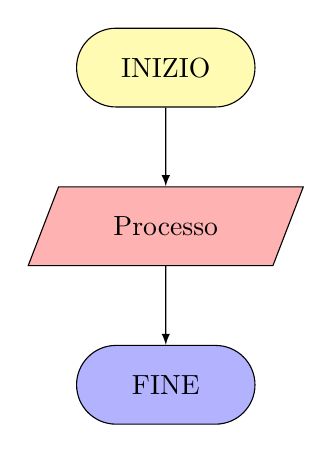
\begin{tikzpicture}
					% Start block
					\node[draw,
					rounded rectangle,
					fill=yellow!30,
					minimum width=2.5cm,
					minimum height=1cm] (block1) {INIZIO};
					% Process block
					\node[draw,
					trapezium, 
					trapezium left angle = 65,
					trapezium right angle = 115,
					trapezium stretches,
					fill=red!30,
					below=of block1,
					minimum width=3.5cm,
					minimum height=1cm
					] (block2) { Processo };
					% End block
					\node[draw,
					rounded rectangle,
					fill=blue!30,
					below=of block2,
					minimum width=2.5cm,
					minimum height=1cm] (block3) {FINE};
					% Arrows
					\draw[-latex] (block1) edge (block2)
					(block2) edge (block3);
					\end{tikzpicture}
				\end{multicols}
			\end{center}
	\newpage
		\section{Dove e perchè viene usato \LaTeX}
		\LaTeX\space viene usato da fisici, matematici, ricercatori ed ingegneri, ed è diventato lo \textbf{standard nel mondo accademico}. Inoltre, la maggior parte delle multinazionali richiedono l'invio del CV in questo formato.
		\\É un linguaggio che \textbf{richiede una certa pratica}, ma permette di creare construtti che sarebbero impossibili da creare con qualsiasi altro programma, e fa tutto ciò in un ambiente unico. Ad esempio gli spartiti musicali vengono scritti utilizzando un "ramo" di \LaTeX\space chiamato \textsc{MusiXTEX}.
		\\Nel mondo della matematica viene usato per scrivere facilmente formule, disegnare grafici e diagrammi.
		\\Alcuni componenti di \textsc{WikipediA} sono scritti in \LaTeX\space, come le formule matematiche e le formule chimiche.
		\\In conclusione, \LaTeX\space \textbf{permette di fare cose altrimenti impossibili con altri programmi}, e ne è la conferma il suo stesso logo. 
	
		\section{Dove scaricare \LaTeX}
		\LaTeX\space è gratuito ed è disponibile per ogni tipo di sistema operativo. Per scaricarlo basta recarsi alla seguente pagina web e cliccare su "Download Now".
		\\ \url{https://www.texstudio.org}\\
		Un'altro componente necessario è \textbf{MikTEX}. Per scaricarlo è necessario recarsi alla seguente pagina web e scegliere il proprio sistema operativo e scaricare l'installer cliccando sul tasto "Download".
		\\ \url{https://miktex.org/download}\\
	
		\section{Come installare \LaTeX}
	
	
	\chapter{L'interfaccia di TeXstudio}
	In questo capitolo verranno spiegate le principali funzioni di TeXstudio.
		\section{I pannelli}
		L'interfaccia di TeXstudio è divisa in \textbf{4 parti principali}:
			\begin{figure}[h]
				\includegraphics[width=\textwidth]{Chap2/FullTEX.png}
			\end{figure}
	\newpage
	
		\section{Il pannello di testo}
			\begin{figure}[h]
				\includegraphics[width=\textwidth]{Chap2/MainPanel.png}
			\end{figure}
		\noindent Questo è il pannello principale, \textbf{tutto ciò che verra scritto al suo interno sarà "tradotto" nel documento finale}, in maniera analoga a quella del pannello principale di visual studio.\\
		Questo pannello presenta una barra laterale delle scorciatoie, evidenziata in rosso, personalizzabile. Sono presenti opzioni di formattazione, di allineamento testo ed alcuni comuni comandi matematici.\\
		In alto è presente una barra che permette di selezionare diversi documenti, mentre a sinistra del testo è presente un'ulteriore barra, nella quale possono essere inseriti dei marcatori per organizzare meglio il testo e le varie sezioni del documento possono essere contratte.\\
		All'interno di questa barra vengono anche inseriti dei segnalini, per evidenziare la linea da modificare in caso di errori.
	\newpage
	
		\section{Il pannello di output}
		\begin{figure}[h]
			\includegraphics[width=\textwidth]{Chap2/OutputPanel.png}
		\end{figure}
		\noindent In questo pannello viene visualizzato un pdf del documento che è stato scritto nel pannello principale. Infatti, premendo il tasto "Build \& View", o utilizzando la scorciatoia \keystroke{F5}
		, è possibile \textbf{compilare il documento}, così come si compilerebbe un programma su visual studio.\\
		Le modifiche, quindi, \textbf{non sono applicate in tempo reale}, ma vengono mostrate solo una volta che si è compilato il documento. Sono presenti alcuni comandi legati alla visualizzazione del pdf, zoom e scroll, tra i quali ne spicca uno molto utile, che permette di andare alla sorgente di una parola, per vedere il comando che la genera \menu[,]{Tasto Destro,{Go to source}}.
		\newpage
		
		\section{Attrezzi e Scorciatoie}
		\begin{figure}[h]
			\includegraphics[width=\textwidth]{Chap2/ShortcutPanel.png}
		\end{figure}
		\noindent In questo pannello sono presenti alcuni comandi che possono sembrarci familiari, in ordine da destra a sinistra:
		\begin{itemize}
			\item \textbf{New:} crea un nuovo documento;
			\item \textbf{Open:} apre un documento già creato;
			\item \textbf{Save:} sovrascrive l'ultimo salvataggio, o, se premuto per la prima volta, apre una finestra di explora file per selezionare una directory e il nome con cui salvare il documento;
			\item \textbf{Close:} salva e chiude il documento attuale;
			\item \textbf{Undo:} ripristina l'ultima modifica;
			\item \textbf{Redo:} ripristina l'ultimo utilizzo di undo;
			\item \textbf{Copy:} copia il testo selezionato;
			\item \textbf{Cut:} copia e rimuove il testo selezionato;
			\item \textbf{Paste:} incolla l'ultimo testo copiato;
			\item \textbf{Build \& View:} compila e aggiorna il pdf del documento;
			\item \textbf{Build:} compila il documento;
			\item \textbf{Stop Compile:} ferma il processo di compilazione del documento;
			\item \textbf{View:} aggiorna il pdf, mostrando l'ultima compilazione;
			\item \textbf{View Log:} mostra il log nel pannello "Terminale e Log";
			\item \textbf{Scorciatoie:} una serie di scorciatoie, usate per velocizzare la stesura di un documento;
		\end{itemize}		
		\chapter{Creare un nuovo documento}
		Per creare un documento è e necessario premere sul tasto "New". Alternativamente, se si desidera modificare un modello, in inglese "template", è necessario aprire il menù "File" nella parte in alto a sinistra dello schermo e selezionare "Nuovo da Modello".
		\begin{figure}[h]
			\centering
			\includegraphics[scale=0.7]{Chap3/NuovoDaModello.png}
		\end{figure}
		
	\chapter{Le parti principali di un documento}
	Un documento è diviso in due parti principali: la selezione dei pacchetti e la stesura del documento.
	\\\noindent Analizziamo le due parti:
	\section{La selezione dei pacchetti}
	La prima parte del file tex viene utilizzata per elencare le librerie di comandi che verranno usate all'interno del documento, in maniera analoga alle librerie utilizzate in C++. I comandi sono i seguenti:
	\subsection{DocumentClass}
	Il comando DocumentClass viene usato per decidere una serie di opzioni del documento, come la dimensione del testo o la tipologia di documento.
	\\Alcune opzioni sono:
	\begin{itemize}
		\item 12pt: Imposta la dimensione del testo standard a 12.
		\item a4paper: Imposta la dimensione delle pagine ad a4.
		\item openany: Fa si che i capitoli possano trovarsi sia nelle pagine pari che nelle pagine dispari. Permette di evitare pagine vuote all'interno dei documenti.
	\end{itemize}
	La seconda parte del programma permette di decidere la tipologia di documento che si vuole scrivere.
	\\Alcune tipologie sono:
	\begin{itemize}
		\item book: L'opzione standard. Permette di dividere il documento in paragrafi e di aggiungere un indice.
		\item letter: Crea un documento utilizzando un formato adatto ad una lettera.
		\item article: Crea un documento con un formato adatto ad un articolo di giornale
	\end{itemize}
	La sintassi del comando è la seguente:
	\begin{lstlisting}
		\documentclass[opzione, opzione, ...]{tipologia}
	\end{lstlisting}
	
	
	
	\chapter{Organizzare un documento}
	Attraverso diversi comandi possiamo formattare il nostro documento. In genere un testo avrà una pagina di copertina, sulla quale ci sarà scritto il titolo, l'autore e la data. In seguito è possibile inserire un indice "cliccabile", in modo da poter elencare le parti, i capitolo e le sezioni che comporranno il documento.
	\section{Titolo}
	Vediamo più nel dettaglio ogni comando legato al titolo:
	
	\begin{itemize}
		\item \textbf{$\backslash$title\{ Il Mio Documento \LaTeX \}:} Questo comando imposta il titolo del documento.
		
		\item \textbf{$\backslash$author\{ Il Tuo Nome \}:} Questo comando imposta l'autore del documento.
		
		\item \textbf{$\backslash$date\{$\backslash$today\}:} Questo comando imposta la data del documento. In questo caso, è impostato su $\backslash$today per visualizzare la data corrente, ma è possibile inserire una data specifica.
		
		\item \textbf{$\backslash$maketitle:} Questo comando crea il titolo del documento utilizzando le informazioni fornite con $\backslash$title, $\backslash$author, e $\backslash$date.
		
	\end{itemize}
	
	Ogni comando serve a definire aspetti specifici del titolo, dall'identificazione del tipo di documento e la sua codifica, alla formattazione e all'inclusione di informazioni come il titolo, l'autore e la data. Personalizzando questi comandi, è possibile adattare il titolo del tuo documento in modo specifico.
	\newpage
	
	\section{Capitoli, Sezioni e Paragrafi}
	
	Con \LaTeX è possibile dividere un documento in diverse sezioni, con una gerarchia particolare. I comandi sono i seguenti:
	
	\begin{itemize}
		
		\item \textbf{$\backslash$part\{Titolo della Parte\}:} Il comando $\backslash$part viene utilizzato per suddividere un documento in parti. Questo è il "livello" più alto, crea una pagina con all'interno il "Titolo della Parte". Resta spesso inutilizzato.
		
		\item \textbf{$\backslash$chapter\{Titolo del Capitolo\}:} Il comando $\backslash$chapter è utilizzato per iniziare un nuovo capitolo nel documento.
		
		\item \textbf{$\backslash$section\{Titolo della Sezione\}:} Il comando $\backslash$section divide il documento in sezioni all'interno di un capitolo.
		
		\item \textbf{$\backslash$subsection\{Titolo della Sottosezione\}:} Il comando $\backslash$subsection viene utilizzato per suddividere ulteriormente una sezione in sottosezioni.
		
		\item \textbf{$\backslash$subsubsection\{Titolo della Sottosottosezione\}:} Il comando $\backslash$subsubsection suddivide ulteriormente una sottosezione in sottosottosezioni.
		
		\item \textbf{$\backslash$paragraph\{Titolo del Paragrafo\}:} Il comando $\backslash$paragraph viene utilizzato per iniziare un nuovo paragrafo.
		
		\item \textbf{$\backslash$subparagraph\{Titolo del Sottoparagrafo\}:} Il comando $\backslash$subparagraph viene utilizzato per suddividere ulteriormente un paragrafo.
		
	\end{itemize}
	Questo è un esempio di come organizzare la struttura di un documento. si può adattare e personalizzare queste strutture in base alle esigenze del tuo documento.
	\begin{lstlisting}
		\documentclass{book}
		\begin{document}
			
			\part{Parte}
			\chapter{Capitolo}
			\section{Sezione}
			\subsection{Sottosezione}
			\subsubsection{SottoSottosezione}
			\paragraph{Paragrafo}
			\subparagraph{Sottoparagrafo}
			
			\chapter{Secondo Capitolo}
			\section{Sezione}
			\section{Seconda Sezione}
			
			\part{Seconda Parte}
			\chapter{Primo Capitolo}
			\section{Prima Sezione}
			
		\end{document}
	\end{lstlisting}
	\textbf{All'interno della cartella sorgente di questo documento è presente una cartella con all'interno degli esempi. Per vedere un documento di esempio riguardo questo argomento, apri il seguente file:}
	\menu{Guida LaTeX>Esempi>Organizzazione1>Organizzazione1.pdf}
	\newpage
	
	\section{Formattazione in più colonne}
	
	Il pacchetto multicol in LaTeX consente di creare un ambiente a più colonne nel tuo documento. Di seguito, la spiegazione di come utilizzare l'ambiente multicols e una descrizione dei principali comandi ad esso associati.
	
	\begin{itemize}
		\item\textbf{$\backslash$begin\{multicols\}\{NumeroColonne\}:} Questo comando inizia l'ambiente a più colonne, specificando il numero di colonne desiderato.
		
		\item \textbf{$\backslash$end\{multicols\}:} Questo comando termina l'ambiente a più colonne.
		
		\item \textbf{$\backslash$columnbreak:} Questo comando forza un'interruzione di colonna, spostando il contenuto sulla colonna successiva.
		
		\item \textbf{$\backslash$columnsep:} Questo comando imposta la larghezza del separatore verticale tra le colonne. si può modificarlo secondo le tue preferenze.
		
		\item \textbf{$\backslash$setlength\{$\backslash$multicolsep\}\{value\}:}	
		Questo comando imposta lo spazio verticale aggiunto tra le colonne. Modifica "value" secondo le tue preferenze.
	\end{itemize}
	\begin{lstlisting}
		\documentclass{article}
		\usepackage{multicol}
		
		\begin{document}
			
			\begin{multicols}{2}
				% Contenuto della prima colonna
				Questo e il contenuto della prima colonna.
				puoi inserire testo, formule matematiche, immagini, ecc.
				
				\columnbreak % Sposta il contenuto sulla seconda colonna
				
				% Contenuto della seconda colonna
				Questo e il contenuto della seconda colonna.
				puoi personalizzare il layout in base alle tue esigenze.
			\end{multicols}
			
		\end{document}
		
	\end{lstlisting}
	\newpage
	\section{Elenchi puntati, numerati e personalizzati}
	\subsection{Elenchi puntati}
	Per creare un elenco puntato in LaTeX, si può utilizzare l'ambiente \textbf{itemize}. Ecco un esempio:	
	\begin{lstlisting}
		\begin{itemize}
			\item Primo elemento
			\item Secondo elemento
			\item Terzo elemento
		\end{itemize}
	\end{lstlisting}
	Questo produrrà un elenco puntato con pallini.
	\subsection{Elenchi numerati}
	Per creare un elenco numerato in LaTeX, si può utilizzare l'ambiente \textbf{enumerate}. Ecco un esempio:
	\begin{lstlisting}
		\begin{enumerate}
			\item Primo elemento
			\item Secondo elemento
			\item Terzo elemento
		\end{enumerate}
	\end{lstlisting}
	Questo produrrà un elenco numerato con numeri arabi.
	\subsection{Elenchi personalizzati}
	si può personalizzare i simboli dell'elenco puntato o numerato utilizzando il pacchetto \textbf{enumitem}. Ecco un esempio:
	\begin{lstlisting}
		\usepackage{enumitem}
		
		\begin{document}
			
			\begin{itemize}[label=$\diamond$]
				\item Primo elemento
				\item Secondo elemento
				\item Terzo elemento
			\end{itemize}
			
			\begin{enumerate}[label=(\alph*)]
				\item Primo elemento
				\item Secondo elemento
				\item Terzo elemento
			\end{enumerate}
			
		\end{document}
	\end{lstlisting}
	In questo esempio, l'elenco puntato utilizza il simbolo del diamante, mentre l'elenco numerato utilizza lettere minuscole tra parentesi.
	\\
	si può personalizzare ulteriormente gli elenchi con le opzioni fornite dal pacchetto \textbf{enumitem}, come ad esempio regolare il margine sinistro, la distanza tra gli elementi, ecc.
	
	
	
	
	
	\chapter{Le formule matematiche}
	\section{Inizializzare una formula matematica}
	\subsection{Inserire Modalità Matematica Inline:}
	Per inserire espressioni matematiche all'interno del testo, si può utilizzare la modalità matematica inline tra dollari $...$:
	\begin{lstlisting}Il teorema di Pitagora afferma che $a^2 + b^2 = c^2$.\end{lstlisting}
	\begin{lstlisting}
		\begin{equation}
			\int_{a}^{b} f(x) \,dx = F(b) - F(a)
		\end{equation}
	\end{lstlisting}
	\subsection{Ambienti Matematici Avanzati:}
	Per espressioni matematiche più complesse, si può utilizzare ambienti come align per allineare equazioni:
	\begin{lstlisting}
		\begin{align}
			2x + 3y &= 8 \\
			4x - y &= 2
		\end{align}
	\end{lstlisting}
	
	
	
	\section{Operatori e simboli matematici}
	\subsection{Parentesi automatiche}
	In LaTeX, il dimensionamento automatico delle parentesi può essere gestito tramite i comandi $\backslash$left e $\backslash$right. Questi comandi vengono utilizzati per delimitare espressioni matematiche con parentesi, graffe, parentesi quadre, ecc., e adattano automaticamente le dimensioni delle parentesi alla dimensione dell'espressione al loro interno.
	\\
	Ecco un esempio di utilizzo di $\backslash$left e $\backslash$right con parentesi tonde:
	\begin{lstlisting}
		\begin{document}	
			\[ \left( \frac{a}{b} \right) \]				
		\end{document}
	\end{lstlisting}
	Si può anche utilizzare $\backslash$left e $\backslash$right con altri delimitatori come graffe {}, parentesi quadre [], barre verticali, ecc.
	
	
	
	\subsection{Frazioni}
	Il comando $\backslash$dfrac è una versione di $\backslash$frac (utilizzato per scrivere frazioni) fornito dal pacchetto amsmath che rende automaticamente il numeratore e il denominatore con dimensioni display, rendendo la frazione più adatta per la visualizzazione in formule più grandi, come in modalità display matematica o nelle tabelle.
	\\
	Ecco un esempio di come si può utilizzare $\backslash$dfrac:
	\begin{lstlisting}
		\usepackage{amsmath}
		
		\[ \dfrac{a}{b} \]
	\end{lstlisting}
	Nel contesto di un'espressione più complessa o di un ambiente di visualizzazione matematica, $\backslash$dfrac può essere utile per migliorare l'aspetto delle frazioni.
	
	\subsection{Apici e pedici}
	Per aggiungere apici e pedici in LaTeX, si può utilizzare i simboli \textunderscore (underscore) per il pedice e \textasciicircum (caret) per l'apice. Ecco alcuni esempi:
	\begin{lstlisting}
		\[ a_{1} \] % Pedice
		\[ b^{2} \] % Apice
		\[ c_{1}^{2} \] % Pedice e Apice combinati
	\end{lstlisting}
	Da notare che tutti gli altri comandi funzionano correttamente anche all'interno di apici e pedici:
	\begin{lstlisting}
		\[ a_{\sqrt{10}} \] % Pedice radice 10
		\[ b^{\exp{\pi}} \] % Apice esponenziale pigreco
	\end{lstlisting}
	
	\subsection{Radicali}
	Per scrivere radicali in LaTeX, è necessario utilizzare il comando $\backslash$sqrt. Si può anche personalizzare il grado della radice quadrata utilizzando $\backslash$sqrt[n]{x}, dove $n$ rappresenta l'ordine della radice.
	\\
	Ecco alcuni esempi:
	\begin{lstlisting}
		\begin{document}	
			\[ \sqrt{2x+1} \] % Radice quadrata di 2x+1
			\[ \sqrt[3]{8} \] % Radice cubica di 8
			\[ \sqrt[n]{x} \] % Radice n-esima di x
		\end{document}
	\end{lstlisting}
	
	\subsection{Esponenziali}
	Per scrivere la funzione esponenziale in LaTeX, si può utilizzare il comando $\backslash$exp.\\
	Ecco alcuni esempi:
	\begin{lstlisting}
		\begin{document}					
			\[ y = \exp(x) \]					
			\[ y = \exp(2x + 1) \]
		\end{document}
	\end{lstlisting}
	Il comando $\backslash$exp rappresenta la funzione esponenziale e può essere utilizzato all'interno di espressioni matematiche più complesse. Se desideri scrivere la funzione esponenziale elevata a una potenza specifica, puoi usare il comando "apice":
	\begin{lstlisting}
		\begin{document}					
			\[ y = \exp(x^2) \]					
		\end{document}
	\end{lstlisting}
	
	\subsection{Funzioni trigonometriche}
	Per scrivere le funzioni trigonometriche di base, è necessario utilizzare i comandi seguenti:
	\begin{lstlisting}
		\begin{document}					
			\sin(x)		%seno
			\cos(x)		%coseno
			\tan(x)		%tangente
			
			\arcsin(x)	%arcoseno
			\arccos(x)	%arcocoseno
			\arctan(x)	%arcotangente
			
			\sec(x)		%secante
			\csc(x)		%cosecante
			\cot(x)		%cotangente
		\end{document}
	\end{lstlisting}
	
	\subsection{Sommatorie}
	Per scrivere sommatorie in LaTeX, si può utilizzare il comando $\backslash$sum. Ecco alcuni esempi di come potresti rappresentare sommatorie di base:
	\begin{lstlisting}
		\begin{document}					
			\sum_{i=1}^{n} a_i	%sommatoria di a_i da 1 a n
			
			\sum_{k=0}^{\infty} \frac{1}{2^k} %sommatoria infinita di 1 diviso 2^k
		\end{document}
	\end{lstlisting}
	
	\subsection{Integrali}
	Per scrivere integrali in LaTeX, si può utilizzare il comando $\backslash$int. Ecco alcuni esempi di come rappresentare integrali di base:
	\begin{lstlisting}
		\begin{document}					
			\int_{a}^{b} f(x) \,dx 	%integrale definito della funzione f(x) da a a b
			
			\int f(x) \,dx 			%integrale indefinito della funzione f(x)
		\end{document}
	\end{lstlisting}

	\subsection{I Limiti}
	Per scrivere limiti in LaTeX, si può utilizzare il comando  $\backslash$lim. Ecco alcuni esempi di come rappresentare limiti di base:
	\begin{lstlisting}
		\begin{document}					
			\lim_{x \to a} f(x)			%limite finito
			\lim_{x \to \infty} g(x)	%limite infinito
			\lim_{x \to a^+} h(x)		%limite laterale destro
			\lim_{x \to a^-} k(x)		%limite laterale sinistro
		\end{document}
	\end{lstlisting}
	\newpage
	\subsection{Le lettere greche}
	Per scrivere lettere greche in LaTeX, puoi utilizzare i comandi corrispondenti per ciascuna lettera greca. Ecco una lista delle lettere greche comuni e i comandi corrispondenti:
	\begin{multicols}{2}
		\begin{itemize}
			\item     Alpha:  $\backslash$alpha
			\item     Beta: $\backslash$beta
			\item     Gamma: $\backslash$gamma
			\item     Delta: $\backslash$delta
			\item     Epsilon: $\backslash$epsilon
			\item     Zeta: $\backslash$zeta
			\item     Eta: $\backslash$eta
			\item     Theta: $\backslash$theta
			\item     Iota: $\backslash$iota
			\item     Kappa: $\backslash$kappa
			\item     Lambda: $\backslash$lambda
			\item     Mu: $\backslash$mu
			\item     Nu: $\backslash$nu
			\item     Xi: $\backslash$xi
			\item     Omicron: $\backslash$omicron
			\item     Pi: $\backslash$pi
			\item     Rho: $\backslash$rho
			\item     Sigma: $\backslash$sigma
			\item     Tau: $\backslash$tau
			\item     Upsilon: $\backslash$upsilon
			\item     Phi: $\backslash$phi
			\item     Chi: $\backslash$chi
			\item     Psi: $\backslash$psi
			\item     Omega: $\backslash$omega
		\end{itemize}
		\columnbreak
		\begin{itemize}
			\item     Alpha:  $\backslash$Alpha
			\item     Beta: $\backslash$Beta
			\item     Gamma: $\backslash$Gamma
			\item     Delta: $\backslash$Delta
			\item     Epsilon: $\backslash$Epsilon
			\item     Zeta: $\backslash$Zeta
			\item     Eta: $\backslash$Eta
			\item     Theta: $\backslash$Theta
			\item     Iota: $\backslash$Iota
			\item     Kappa: $\backslash$Kappa
			\item     Lambda: $\backslash$Lambda
			\item     Mu: $\backslash$Mu
			\item     Nu: $\backslash$Nu
			\item     Xi: $\backslash$Xi
			\item     Omicron: $\backslash$Omicron
			\item     Pi: $\backslash$Pi
			\item     Rho: $\backslash$Rho
			\item     Sigma: $\backslash$Sigma
			\item     Tau: $\backslash$Tau
			\item     Upsilon: $\backslash$Upsilon
			\item     Phi: $\backslash$Phi
			\item     Chi: $\backslash$Chi
			\item     Psi: $\backslash$Psi
			\item     Omega: $\backslash$Omega
		\end{itemize}
	\end{multicols}
	
	\section{I Sistemi}
	Per scrivere sistemi di equazioni in LaTeX, si può utilizzare l'ambiente \textbf{cases} fornito dal pacchetto \textbf{amsmath}. Ecco un esempio di come rappresentare un sistema di due equazioni:
	\begin{lstlisting}
	\begin{equation}
		\begin{cases}
			2x + 3y = 6 \\
			4x - y = 5
		\end{cases}
	\end{equation}
	\end{lstlisting}
	Questo produrrà un sistema di due equazioni all'interno di parentesi graffe.
	\\
	Per cambiare il tipo di parentesi intorno al sistema di equazioni in LaTeX, si può utilizzare il pacchetto \textbf{empheq}.\\
	Questo pacchetto offre una maggiore flessibilità nella personalizzazione degli ambienti di equazione. Ecco un esempio:
	\begin{lstlisting}
	\begin{empheq}[left=\begin{Bmatrix}, right=\end{Bmatrix}]{equation}
		\begin{aligned}
			2x + 3y &= 6 \\
			4x - y &= 5
		\end{aligned}
	\end{empheq}
	\end{lstlisting}
	In questo esempio sono state utilizzate le parentesi graffe "Bmatrix" come delimitatori del sistema di equazioni.\\
	Puoi sostituire Bmatrix con i seguenti delimitatori a seconda delle tue preferenze. 
	\begin{itemize}
		\item \textbf{matrix:} vuoto
		\item \textbf{pmatrix:} parentesi tonde
		\item \textbf{bmatrix:} parentesi quadre
		\item \textbf{Bmatrix:} parentesi graffe
		\item \textbf{vmatrix:} righe verticali
		\item \textbf{Vmatrix:} righe verticali doppie
	\end{itemize}
	
	
	\section{Le Matrici}
	\section{Le Tabelle}
	
	
	
	
	
	
	
	
\end{document}